\section{Results}
We evaluated approximately 650 sentences per condition. The basic statistics of the results are included in Table~\ref{stats}. It's unclear which of these statistics is the most important measure

\begin{table}
\centering
\begin{tabular}{l|ccc}
Condition & Mean & Median & Variance \\
Early & $10^{-5}$ & $10^{-11}$ & $10^{-7}$ \\ \hline
Middle & $10^{-7}$ & $10^{-11}$ & $10^{-11}$ \\
Late & $10^{-7}$ & $10^{-10}$ & $10^{-11}$ \\
Default & $10^{-7}$ & $10^{-10}$ & $10^{-11}$ \\
Control & $10^{-5}$ & $10^{-20}$ & $10^{-6}$ \\
\end{tabular}
\label{stats}
\caption{Recall that a higher probability means that those sentences are more likely. Due to the size of the numbers, only the order of magnitude is included.}
\end{table}

After confirming that the distributions were very far from normal, we proceeded with pairwise Wilcox tests, which can be seen in Table~\ref{result}.

\begin{table}
\centering
\begin{tabular}{l|cc}
Condition-Pair & w-score & p-value \\ \hline
Early-Default & 160050 & $<0.00001$ \\
Early-Control & 499320 & $<0.00001$ \\
Early-Middle & 2238700 & $0.1702$ \\
Early-Late & 177950 & $<0.00001$ \\
Middle-Late & 177950 & $<0.00001$ \\
Middle-Default & 161410 & $<0.00001$ \\
Middle-Control & 493680 & $<0.00001$ \\
Default-Late & 229670 & $0.0342$ \\
Default-Control & 541230 & $<0.00001$ \\
Late-Control & 545950 & $<0.00001$ 
\end{tabular}
\label{result}
\caption{The results of the pairwise Wilcox tests. The null hypothesis is that the two samples are drawn from the same distribution.}
\end{table}

The Wilcox test is determining what the probability is that two sets of samples could have been drawn from the same distribution. From this, we can conclude that the Early results are notably different than those for Default and Control. On the other hand, Early is not reliably different than Middle. The basic pattern of this suggests that there are three basic groups. Control is notably the best, which of course is not surprising, as it should be seen as an asymptote models hope to approach. Then, Early and Middle pattern together, while Default and Late pattern together. 

This of course, is fairly unsatisfying without some sort of ordering. It's impossible to get a perfectly valid comparison among statistics from this type of methodology; however, by looking at the simple statistics, we can vaguely conclude that Early is performing the best. Its values for mean, median, and variance are all closer to Control than the other conditions. Alternatively, we can look at the actual w-scores. While it is not intended to be used as a distance metric for distributions, a higher value means it's less probable the samples are from the same distribution. Along this metric, Early and Middle outperform Late and Default. 

\subsection{Branching Factor}
The branching factor, as explained earlier, could help pinpoint the exact difference between the conditions. In other words, since our analysis relied on a heuristic, measuring the branching factor of the sentences produced checks if they are measuring what we expect. If there was no systematic bias in sentence production, we would expect Early to be more right-branching, Late to be more left-branching, and Middle and Default to both be about even. 

Our process was fairly simple, looking at the order of combination and if left- or right-branching trees were being formed. An example tree is shown in Figure~\ref{tree}. The numbers represent the branching factors of each sub-tree. Branching factors are computed by weight: if a tree has more nodes in its left sub-tree, then it is more right-branching. The total branching factor is based on the sum of each of these subtrees. An alternative metric of branching factor just computes what percentage of branches are right-branching. This considers something right-branching if a larger tree to the left absorbs a smaller tree to the right. This naturally correlates very well with the previous metric. Both metrics per condition are displayed in Table~\ref{bfmem}. 

\subsection{Working Memory Load}
We expect a realistic process of sentence production to try to minimize cognitive load. We have an approximate measure of the working memory load from the trace of the process; however, it is important to recognize that it is fairly limited in its usefulness. While this does represent the memory of the syntactic process, it does not represent the memory of the semantic process. Typically, we assume a right-branching process will take less working memory, because semantic and lexical items can be retrieved as they are needed. However, in terms of syntax, a purely right-branching process and a purely left-branching process will take an equivalent amount of memory. This relationship can be fairly clearly displayed in Table~\ref{bfmem}. Nonetheless, we see an interesting phenomenon emerge, where the two cases that pattern together in ngram scores also pattern together in working memory load.

\begin{figure}[ht]
\begin{center}
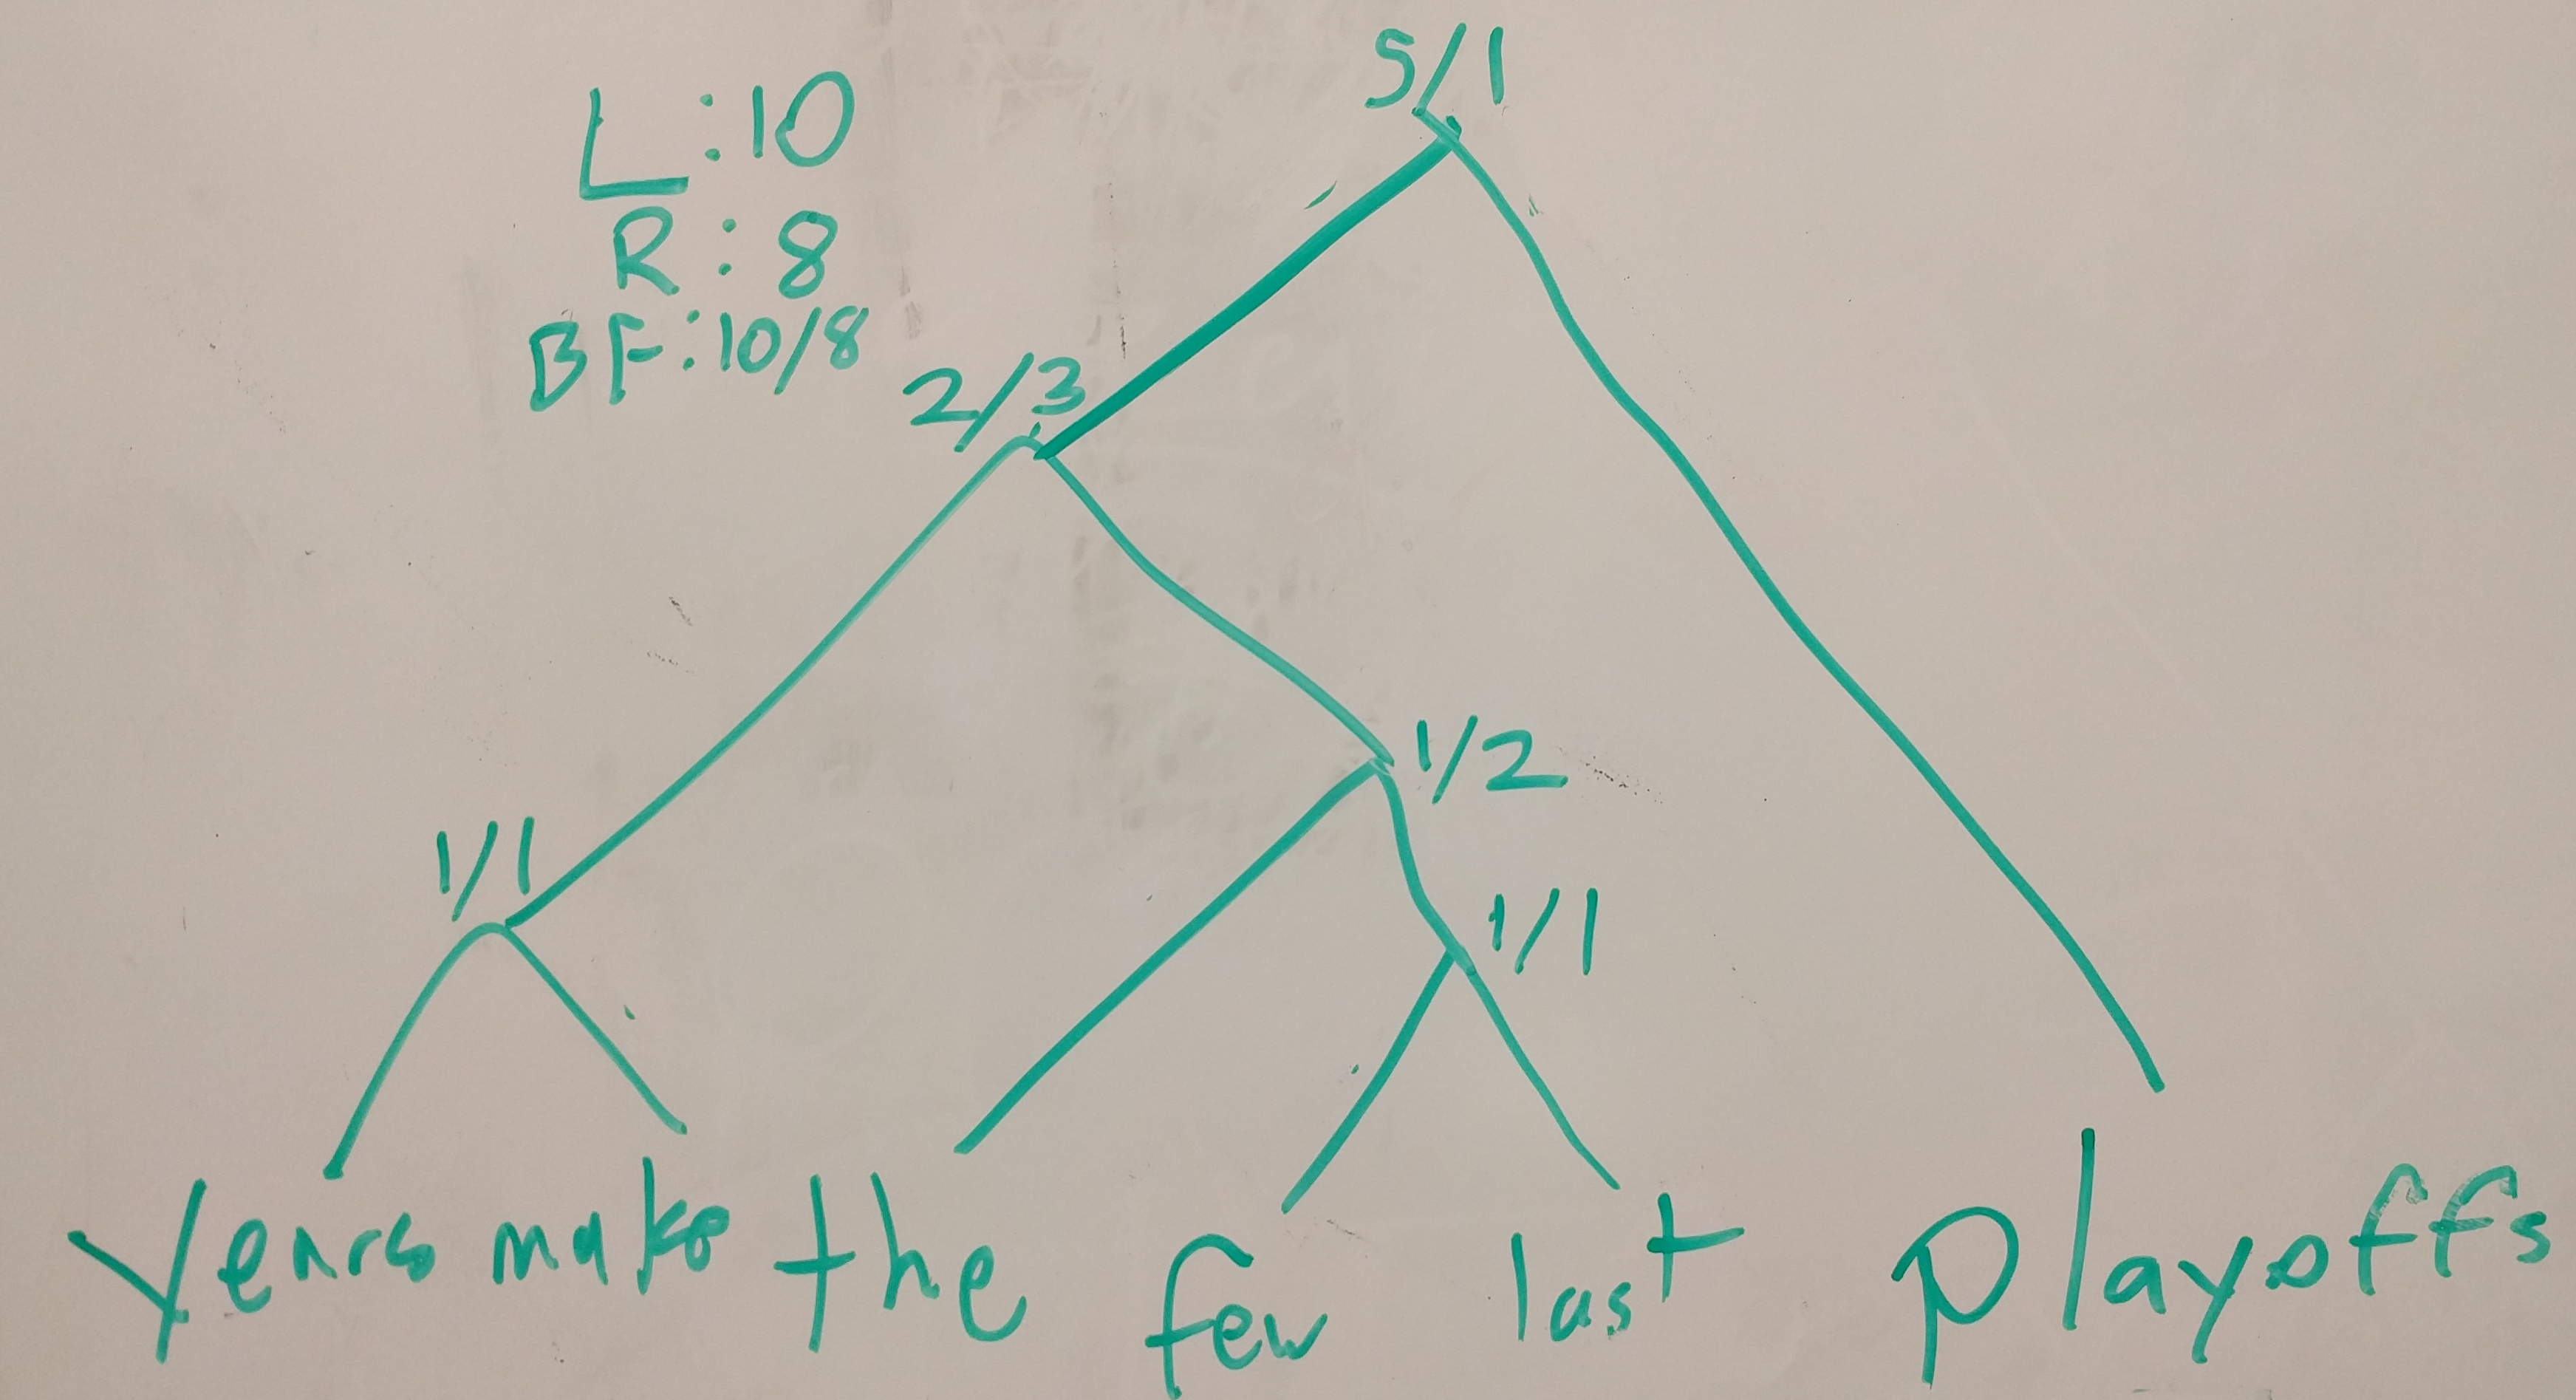
\includegraphics[width=0.95\columnwidth]{figures/tree}
\end{center}
\caption{An example of the syntax tree of actual output from the model. The overall branching factor of this tree is 10/8, or 1.25, indicating that it is primarily right-branching. This means that this tree represents a more incremental process.\textbf{temp diagram}}  
\label{tree}
\end{figure}

\begin{table}
\centering
\begin{tabular}{l|cccc}
Condition & RBF & RBF-alt & WM-eff & WM-avg \\ \hline
Early & 0.811 & 0.065 & 1.931 & 2.915 \\
Middle & 1.276 & 0.283 & 1.964 & 2.926 \\
Late & 1.102 & 0.165 & 1.654 & 3.112 \\
Default & 1.124 & 0.164 & 1.646 & 3.255 \\
\end{tabular}
\label{bfmem}
\caption{RBF and RBF-alt refer to the right-branching factor. In both, higher numbers means more right-branches. WM-eff is the average size of sentence produced per working memory used, so higher is better. WM-avg is just how much space is used, so lower is better.}
\end{table}

\subsection{Edit Distance}
Edit distance reflects how closely the model recreated the original sentence. While this is not necessarily the exact goal, it possibly reflects the strategy the models are using to perform better than the others. Further, while our semantic representation is weak, edit distance is a generally good metric to measure performance, as it relates all parts of the realization process. The specific edit distance metric we used is Levenshtein distance, which, due to its flexibility, will less strongly penalize phrases that are misplaced. This means that a low Levenshtein distance could suggest that a model is learning something about word order. Additionally, we looked at what we refer to as \textit{slot-based} edit distance. This simple metric just penalizes a sentence for each time it does not exactly match the input sentence. Lastly, we used the ROUGE metric, a metric originally designed for paraphrase similarity that can be thought of as a metric of semantic similarity \citep{rouge}. ROUGE has three measurements, based on shared ngrams, shared skipgrams, and shared subsequences, respectively. The results of these metrics can be seen in Table~\ref{distance}. 

\begin{table}
\centering
\begin{tabular}{l|ccccc}
Condition & Slot-Based & Leven & ROUGE-N & ROUGE-L & ROUGE-S  \\ \hline
Early & 0.811 & 0.065 & 0.028 & 0.036 & 0.000 \\
Middle & 1.276 & 0.283 & 0.029 & 0.039 & 0.004 \\
Late & 1.102 & 0.165 & 0.017 & 0.031 & 0.003 \\
Default & 1.124 & 0.164 & 0.016 & 0.024 & 0.000 \\
\end{tabular}
\label{distance}
\end{table}